% TODO(team): Edit section inputs and presentation metadata here.
\documentclass[aspectratio=169,12pt]{beamer}
% TODO(team): Adjust shared colors, typography and layout here, not per slide.
\usepackage[T1]{fontenc}
% Heros provides a clean sans-serif family and remains compatible with pdfLaTeX.
\usepackage{tgheros}
\renewcommand{\familydefault}{\sfdefault}
\usefonttheme{professionalfonts}
\usepackage{booktabs,tabularx,array}
\usepackage{tikz}
\usetikzlibrary{positioning,arrows.meta}
\graphicspath{{dist/figures/}{../../results/compact-study/figures/}}
\definecolor{Navy}{HTML}{16324F}
\definecolor{Teal}{HTML}{167D8D}
\definecolor{Orange}{HTML}{D57929}
\definecolor{Pale}{HTML}{EDF3F7}
\setbeamercolor{structure}{fg=Teal}
\setbeamercolor{frametitle}{fg=Navy}
\setbeamercolor{title}{fg=Navy}
\setbeamercolor{block title}{bg=Pale,fg=Teal}
\setbeamercolor{block body}{bg=Pale,fg=Navy}
\setbeamerfont{block title}{series=\bfseries,size=\normalsize}
\setbeamerfont{title}{series=\bfseries,size=\LARGE}
\setbeamerfont{subtitle}{size=\normalsize}
\setbeamerfont{frametitle}{series=\bfseries,size=\large}
\setbeamercolor{normal text}{fg=Navy,bg=white}
\setbeamertemplate{navigation symbols}{}
\setbeamertemplate{itemize items}[circle]
\setbeamersize{text margin left=8mm,text margin right=8mm}
\setbeamertemplate{frametitle}{\vspace{3mm}\insertframetitle\par\nointerlineskip\vskip1.2mm\hbox{\textcolor{Teal}{\rule{12mm}{1.4pt}}}\vspace{1mm}}
\setbeamertemplate{footline}{\hspace{8mm}\scriptsize CS512\enspace|\enspace\insertsectionhead\hfill\insertframenumber\hspace{8mm}\vspace{3mm}}
\setlength{\tabcolsep}{5pt}
\renewcommand{\arraystretch}{1.3}
% Give lists breathing room without introducing per-slide positioning.
\addtobeamertemplate{itemize/enumerate body begin}{\setlength{\itemsep}{3pt}}{}
\newcolumntype{Y}{>{\raggedright\arraybackslash}X}
\newcommand{\takeaway}[1]{\par\vspace{3mm}\vfill\begin{beamercolorbox}[sep=2mm,wd=\textwidth]{block body}\small\textbf{#1}\end{beamercolorbox}}
\newcommand{\evidence}[1]{\par\vspace{2mm}{\scriptsize\color{gray}#1\par}}
\tikzset{box/.style={draw=Teal,fill=Pale,rounded corners=2pt,align=center,minimum height=9mm,font=\small},flow/.style={-{Stealth},thick,draw=Teal},meta/.style={flow,dashed}}

% Keep translated Beamer labels readable in PDF bookmarks.
\pdfstringdefDisableCommands{\def\translate#1{#1}}
\title[Playback and Replica Recovery]{Balancing Playback Continuity\\and Replica Recovery}
\subtitle{Cooperative Video Storage: System and Experimental Findings}
\author{Haoyu \and Yuquan \and Tian}
\institute{COMPSCI 512}
\date{November 14, 2026}
% Change to \showdemofalse to omit the optional demonstration page.
\newif\ifshowdemo
\showdemotrue
% Uncomment for a presenter copy with notes on separate pages:
% \setbeameroption{show notes}
\begin{document}
\begin{frame}[plain]
  \titlepage
  \note{Introduce the team. The contribution is a working application and controlled evidence about repair, not a new consensus algorithm.}
\end{frame}
% TODO(team): Rehearse the architecture explanation and optional real-media demo.
\section{System}
\begin{frame}{One upload budget serves two demands}
\centering
% Use explicit edge anchors and two-line labels in the gaps between boxes.
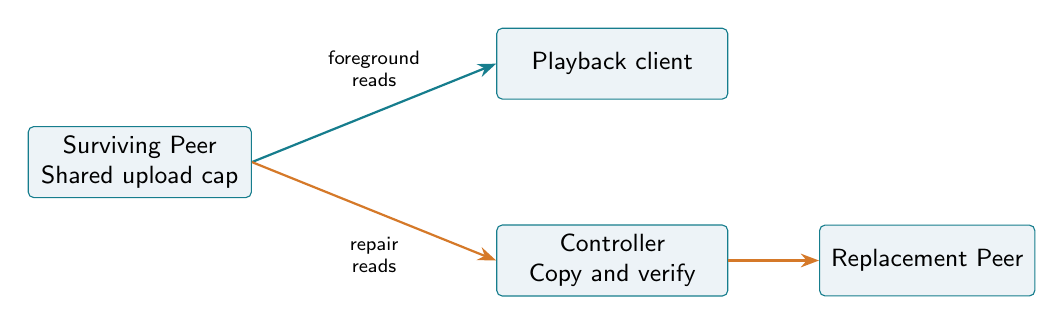
\begin{tikzpicture}
\node[box,text width=26mm] (p) at (0,0) {Surviving Peer\\Shared upload cap};
\node[box,text width=27mm] (v) at (6,1.25) {Playback client};
\node[box,text width=27mm] (c) at (6,-1.25) {Controller\\Copy and verify};
\node[box,text width=25mm] (t) at (10,-1.25) {Replacement Peer};
\draw[flow] (p.east)--node[midway,above=2mm,align=center,font=\scriptsize]{foreground\\reads}(v.west);
\draw[flow,draw=Orange] (p.east)--node[midway,below=2mm,align=center,font=\scriptsize]{repair\\reads}(c.west);
\draw[flow,draw=Orange] (c.east)--(t.west);
\end{tikzpicture}
\takeaway{Repair restores a second source, but consumes bandwidth needed by viewers.}
\note{Conceptual data paths, not a measured traffic trace. The surviving source uploads repair bytes to the Controller, which forwards them to a replacement Peer.}
\end{frame}

\begin{frame}{Control plane and data plane}
\centering
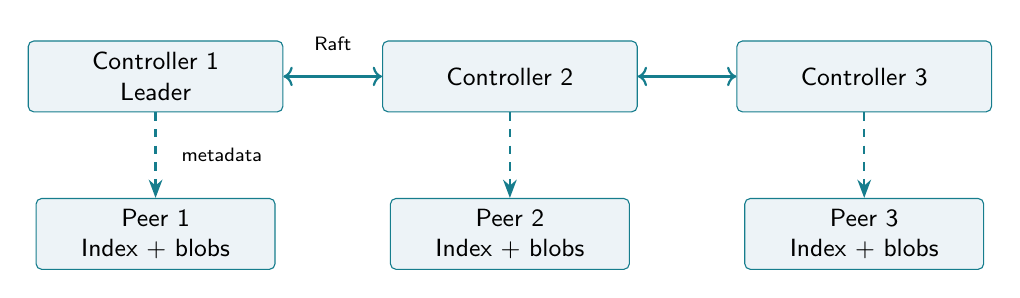
\begin{tikzpicture}
\node[box,text width=30mm] (c1) at (0,0) {Controller 1\\Leader};
\node[box,text width=30mm] (c2) at (4.5,0) {Controller 2};
\node[box,text width=30mm] (c3) at (9,0) {Controller 3};
\draw[flow,<->] (c1)--node[midway,above=2mm,font=\scriptsize]{Raft}(c2);
\draw[flow,<->] (c2)--(c3);
\node[box,text width=28mm] (p1) at (0,-2) {Peer 1\\Index + blobs};
\node[box,text width=28mm] (p2) at (4.5,-2) {Peer 2\\Index + blobs};
\node[box,text width=28mm] (p3) at (9,-2) {Peer 3\\Index + blobs};
\draw[meta] (c1)--node[midway,right=2mm,font=\scriptsize]{metadata}(p1);
\draw[meta] (c2)--(p2);\draw[meta] (c3)--(p3);
\end{tikzpicture}
\small
\begin{itemize}
\item Raft: manifests, committed receipts, publication state, persistent tasks.
\item Browser: Peer $\rightarrow$ Gateway $\rightarrow$ Browser.
\item Experiment: Peer $\rightarrow$ headless client; Gateway is outside Raft.
\end{itemize}
\note{Dashed links indicate control information, not video replication through Raft. Any current leader coordinates maintenance; the vertical links do not assign a Peer to a particular Controller. Peers use independent stores and upload limiters.}
\end{frame}

\begin{frame}{Publish only after two durable copies}
\begin{enumerate}
\item Create a \textbf{DRAFT} manifest.
\item Upload segments; Peers validate size and SHA-256 and persist bytes.
\item Confirm receipts from \textbf{two distinct holders per segment}.
\item Commit \textbf{READY}; expose the video for playback.
\end{enumerate}
\takeaway{Raft commits metadata. Peers store the video bytes outside the Raft log.}
\note{The application checks Peer receipts before publication. Browser playback uses continuous fMP4. Experimental payloads are deterministic bytes with simulated media durations.}
\end{frame}

\begin{frame}{Playback recovery $\neq$ redundancy recovery}
\begin{block}{Foreground recovery}
Peer fails $\rightarrow$ try another holder $\rightarrow$ verify bytes $\rightarrow$ continue delivery.
\end{block}
\begin{block}{Background repair}
Detect shortage $\rightarrow$ grace interval $\rightarrow$ commit task\\
$\rightarrow$ copy and verify $\rightarrow$ commit replacement registration.
\end{block}
\takeaway{Continuing playback does not prove that redundancy has been restored.}
\note{A repaired segment is available from the replacement only after successful installation and registration. If both original holders stop before repair reaches a needed segment, that segment remains unavailable.}
\end{frame}

\begin{frame}{Application implementation and validation}
\small
\begin{tabularx}{\textwidth}{YY}
\toprule Application work & Foundation / tool \\\midrule
Publication and persistent task lifecycle & HashiCorp Raft, BoltDB, snapshots\\
Durable indexes and immutable objects & Go HTTP / filesystem, SHA-256\\
Playback, budgets and experiment harness & FFmpeg / FFprobe for media gates\\
Console: faults, cleanup and video deletion & React and TypeScript\\\bottomrule
\end{tabularx}
\vspace{3mm}
Archived gates: build, static/race, smoke, repair, cleanup, deletion, exact fragment timing and media decoding.
\evidence{Evidence: results/compact-study/validation/gates.json.}
\note{The archived media gates do not establish browser performance in the headless study. Attribute the consensus implementation to HashiCorp rather than presenting it as our own Raft implementation.}
\end{frame}

\ifshowdemo
\begin{frame}{Optional demonstration: from upload to playback}
\begin{enumerate}
\item Start three Controllers and three Peers.
\item Upload a rehearsed short clip; observe packaging and publication.
\item Play the video; inspect per-Peer segment counts.
\item Return to the controlled experimental results.
\end{enumerate}
\takeaway{A functional demonstration and comparative performance evidence are different.}
\note{Prepare an already imported clip and a recording as fallbacks. Avoid an unplanned live failure. No screenshot or recording is fabricated or embedded in this deck.}
\end{frame}
\fi

% TODO(team): Keep policy descriptions aligned with the frozen study configuration.
\section{Questions and policies}
\begin{frame}{Three questions organize the study}
\begin{block}{RQ-A: interference and timing --- E1 / E2}
When does repair interfere with delivery? What does waiting change?
\end{block}
\begin{block}{RQ-B: playback / recovery compromise --- E3 / E4}
Does load-aware repair improve outcomes over fixed controls?
\end{block}
\begin{block}{RQ-C: correctness and recovery --- E4 / E5}
Which application properties survive Peer and Controller failures?
\end{block}
\note{Our contribution is a working application and scoped evidence, not the invention of replication, consensus or throttling.}
\end{frame}
\begin{frame}{Every policy obeys the same total source cap}
\begin{tabularx}{\textwidth}{lY}
\toprule Policy & Treatment \\\midrule
N & No failure: normal-service reference\\
OFF & Failure without repair\\
S & Repair shares the common upload service\\
F25 / F50 & Additional repair caps at 25\% / 50\% of source rate\\
L & Load-aware additional repair allowance\\\bottomrule
\end{tabularx}
\takeaway{An additional cap limits repair; it does not reserve bandwidth or raise capacity.}
\note{Keep the total source limiter fixed in every comparison. This avoids giving the proposed policy additional network resources.}
\end{frame}
\begin{frame}{L reacts to source-local foreground activity}
\begin{columns}[T,onlytextwidth]
\column{.31\textwidth}\begin{block}{Foreground busy}Repair allowance:\\ \textbf{25\%} of source cap.\end{block}
\column{.31\textwidth}\begin{block}{Idle for 2 seconds}Relax allowance to\\ \textbf{100\%}.\end{block}
\column{.31\textwidth}\begin{block}{Task age $>60$ s}Repair allowance floor:\\ at least \textbf{50\%}.\end{block}
\end{columns}
\vspace{5mm}
Updates every 250 ms. Task age is persisted with the committed task.
\takeaway{The 60-second branch was regression-tested, but did not activate in these runs.}
\note{Age is not time since the first fault. The compact performance horizon cannot evaluate the long-age branch empirically.}
\end{frame}

% TODO(team): Keep setup and metric boundaries explicit during presentation.
\section{Method}
\begin{frame}{Independent processes on one shared host}
\small
\begin{tabularx}{\textwidth}{lY}
\toprule Controlled setting & Executed values \\\midrule
Topology & 3 Controllers + 3 Peers; real HTTP/TCP\\
Fixture & 9 distinct 128 KiB segments; 2 logical seconds each\\
Source limits & 96 / 144 / 192 KiB/s\\
Demand & Low: 2 viewers; high: 6; burst arrivals at 0 / 4 / 12 s\\
Client & Window 3; concurrency 2; startup buffer 4 s\\
Timeouts & 8 s per download attempt; 42 s per session\\\bottomrule
\end{tabularx}
\takeaway{Real byte transfer with simulated media consumption, not browser measurement.}
\note{Processes share CPU, RAM, disks and the host network stack. Fresh stores do not flush the OS page cache. Placement is fixed; source selection is round-robin.}
\end{frame}
\begin{frame}{Measure delivery and redundancy together}
\begin{columns}[T,onlytextwidth]
\column{.47\textwidth}
\begin{block}{Executed study}
81 unique runs in 67.9 minutes\\
72 E1--E4 runs + 9 E5 runs\\
396 scheduled viewer outcomes\\
Pilots excluded from estimates
\end{block}
\column{.49\textwidth}
\begin{block}{Outcomes}
Completion and observed stalls\\
Verified two-copy restoration\\
Repair payload\\
One-copy exposure (MiB$\cdot$s)
\end{block}
\end{columns}
\small First fault: 5 s. Observation horizon: 50 s. Recovery target: 40 s after fault. Three paired contexts; two per E4 cell.
\note{Treatment order is randomized and traces are paired. Failed viewers stay in the denominator. Inventory verification is sampled approximately every two seconds, so restoration is bracketed rather than exact.}
\end{frame}

% TODO(team): Show completion beside stall comparisons.
\section{E1: repair interference}
\begin{frame}{Separate Peer loss from repair interference}
\begin{columns}[T,onlytextwidth]
\column{.3\textwidth}\begin{block}{N}No failure.\\Normal-service reference.\end{block}
\column{.3\textwidth}\begin{block}{OFF}Peer fails.\\Repair disabled.\end{block}
\column{.3\textwidth}\begin{block}{S}Same Peer failure.\\Shared repair.\end{block}
\end{columns}
\vspace{5mm}
Compare low and high demand across three paired source-failure contexts.
\takeaway{OFF minus N exposes the fault; S minus OFF isolates the repair treatment.}
\note{The failed holder rotates across all three source capacities. Capacity loss and the client timeout budget can cause failures independently of repair.}
\end{frame}
\begin{frame}{Repair can add stalls under contention}
\begin{tabularx}{\textwidth}{lllY}
\toprule Demand & Policy & Completed & Mean observed stall/viewer \\\midrule
Low & N / OFF / S & 6/6 each & 0.00 s each\\
High & N & 18/18 & 3.20 s\\
High & OFF & 7/18 & 3.24 s\\
High & S & 7/18 & 4.46 s\\\bottomrule
\end{tabularx}
\vspace{3mm}
Slowest-Peer failure: all six viewers finished; repair added \textbf{3.46 s/viewer}.
\takeaway{No added stalls at low demand; context-dependent interference at high demand.}
\note{All-viewer mean paired S minus OFF is +1.22 seconds; individual values are -0.13, +0.33 and +3.46. Early failure can lower observed stalls, so completion must stay visible. Source: compact-study-results.md, E1.}
\end{frame}

% TODO(team): Explain exposure units and the distinction between grace and cancellation.
\section{E2: repair timing}
\begin{frame}{Grace trades early action against unnecessary work}
\begin{itemize}
\item Shared repair policy S; grace of \textbf{1 / 3 / 8 seconds}.
\item Brief absence: original Peer returns after \textbf{4 seconds}.
\item Persistent absence: original Peer stays offline.
\item Measure repair payload and time spent with one reachable copy.
\end{itemize}
\takeaway{Grace controls when repair starts, not whether a started task is cancelled.}
\note{An unavailable Peer is not necessarily permanently lost. Grace can avoid copying data that will soon return, but keeps fewer reachable copies for longer.}
\end{frame}
\begin{frame}{Waiting avoids copies, but extends exposure}
\small
\begin{tabularx}{\textwidth}{lYYY}
\toprule Grace & Brief: repair MiB & Persistent: repair MiB & Persistent exposure MiB$\cdot$s \\\midrule
1 s & 0.125 & 0.750 & 17.42\\
3 s & 0 & 0.750 & 18.24\\
8 s & 0 & 0.750 & 20.20\\\bottomrule
\end{tabularx}
\vspace{4mm}\normalsize
All 54 brief-outage viewer sessions completed.
\takeaway{Persistent exposure increased about 16\% from 1 s to 8 s grace.}
\note{One-second grace copied one 128 KiB segment per brief-outage run. Longer grace avoided that work. Full restoration is not strictly monotonic in every context because source contention and coordinator ticks also matter. Source: compact-study-results.md, E2.}
\end{frame}

% TODO(team): Preserve the negative overall result and censored recovery outcome.
\section{E3: policy comparison}
\begin{frame}{Compare adaptation with credible fixed controls}
\begin{block}{Treatments}S: shared \quad F25: 25\% \quad F50: 50\% \quad L: adaptive\end{block}
\begin{itemize}
\item Steady high demand and burst arrivals.
\item Same content, initial copies, source limits and paired fault trace.
\item Evaluate completion, stalls and verified restoration together.
\end{itemize}
\takeaway{Less observed stall alone does not establish a better policy.}
\note{A policy can reduce foreground interference while delaying redundancy recovery. F50 is a prespecified credible comparator, not selected after inspecting the final results.}
\end{frame}
\begin{frame}{No consistent overall advantage for L}
\small
\begin{tabularx}{\textwidth}{lYYY}
\toprule Policy & Steady stall & Burst stall & Verified by 40 s: steady / burst \\\midrule
S & 4.46 s & 6.18 s & 3/3 \quad 2/3\\
F25 & 4.73 s & 6.28 s & 3/3 \quad 1/3\\
F50 & 4.88 s & 6.20 s & 3/3 \quad 2/3\\
L & 4.33 s & 6.21 s & 3/3 \quad 1/3\\\bottomrule
\end{tabularx}
\vspace{3mm}
All policies: \textbf{7/18} steady and \textbf{9/18} burst completions.\\
F25: one burst run unrecovered at the observation horizon.
\takeaway{The data do not establish a consistent L advantage over F50.}
\note{Mean L minus F50 stall difference is -0.55 seconds under steady demand and +0.01 under bursts. The steady change is driven by one context. One L restoration observation at 40.05 seconds is too close to the target for precise timing claims with two-second sampling.}
\end{frame}
\begin{frame}{A local improvement has a recovery cost}
\small Feasible high-load context: the slowest Peer fails; all six viewers finish.
\vspace{3mm}
\begin{tabularx}{\textwidth}{Yll}
\toprule Metric & F50 & L \\\midrule
Observed stall per viewer & 8.53 s & 6.88 s\\
Verified restoration after fault & 33.99 s & 36.06 s\\
One-copy exposure & 18.82 MiB$\cdot$s & 20.38 MiB$\cdot$s\\\bottomrule
\end{tabularx}
\takeaway{L saved 1.65 s of stalls, but restored redundancy 2.07 s later.}
\note{This is a workload-specific compromise, not dominance or a population estimate. Source: compact-study-results.md, E3.}
\end{frame}

% TODO(team): Keep targeted availability separate from buffered playback and permanent loss.
\section{E4: second-holder failure}
\begin{frame}{Can the replacement serve after both holders stop?}
\begin{enumerate}
\item Stop the first original holder.
\item Wait a fixed \textbf{4 / 14 / 30 seconds}, independent of repair success.
\item Stop the second original holder.
\item Probe a preselected late-queue segment from its replacement.
\end{enumerate}
\small S / F50 / L; two paired contexts per delay. Success requires correct hash \emph{and} committed registration.
\takeaway{A buffered viewer may finish even when fresh delivery is unavailable.}
\note{The probe checks one sentinel, not the whole video. Its late queue position makes repair timing important.}
\end{frame}
\begin{frame}{The selected replacement was not ready in time}
\begin{tabularx}{\textwidth}{lYYY}
\toprule Policy & Second fault +4 s & +14 s & +30 s \\\midrule
S & 0/2 & 0/2 & 0/2\\
F50 & 0/2 & 0/2 & 0/2\\
L & 0/2 & 0/2 & 0/2\\\bottomrule
\end{tabularx}
\vspace{4mm}
All 18 probes were unavailable under the specified success condition.
\takeaway{A boundary was observed; no policy advantage or permanent data loss was established.}
\note{Stopped processes retained their disks. Later delays were not tested. A future completed-repair control should verify replacement availability after every required segment is repaired. Source: compact-study-results.md, E4.}
\end{frame}

% TODO(team): Keep recovery timing origins explicit for E5a/b versus E5c.
\section{E5: Controller recovery}
\begin{frame}{Recovery requires a successful application request}
\small
\begin{tabularx}{\textwidth}{Ylll}
\toprule Case & Passed & Median & Origin \\\midrule
E5a: active delivery & 3/3 & 1.52 s & Leader stop\\
E5b: pending repair & 3/3 & 1.60 s & Leader stop\\
E5c: majority loss & 3/3 & 1.04 s & Quorum restored\\\bottomrule
\end{tabularx}
\vspace{4mm}\normalsize
Fresh quorum-backed metadata, not a health response or Leader role string.
\takeaway{All nine tested Controller scenarios passed the application contract.}
\note{E5c excludes deliberate quorum-isolation time in this table. It includes the startup and election interval after the recorded restore event.}
\end{frame}
\begin{frame}{E5a: fresh metadata recovered during delivery}
\begin{itemize}
\item Stop the current Leader during active delivery.
\item Probe fresh, quorum-backed metadata.
\item Warm and cold uncached sessions completed in all three trials.
\end{itemize}
\begin{block}{Observed recovery after Leader stop}
Median \textbf{1.52 s}; observed range \textbf{1.47--2.74 s}.
\end{block}
\note{Cached playback alone cannot demonstrate Controller availability. The cold-session and fresh-probe checks address that distinction. Source: compact-study-results.md, E5a.}
\end{frame}
\begin{frame}{E5b: committed repair survived Leader loss}
\begin{itemize}
\item Stop the Leader with a committed pending repair task.
\item New Leader retains the \textbf{same task ID and creation time}.
\item Target bytes pass hash validation; replacement registration commits.
\item Controller restart retains task state; source restart retains L configuration.
\end{itemize}
\takeaway{3/3 passed; fresh recovery median 1.60 s, range 1.52--1.97 s.}
\note{This verifies application task continuity in addition to Raft election. A new source process gets a new counter instance ID; counters must not be combined as if continuous.}
\end{frame}
\begin{frame}{E5c: without a majority, writes were refused}
\begin{columns}[T,onlytextwidth]
\column{.47\textwidth}\begin{block}{Stable majority loss}
9/9 valid write attempts returned HTTP 503.\\No success acknowledgments.
\end{block}
\column{.49\textwidth}\begin{block}{After quorum restoration}
Baseline state retained.\\Original operation IDs reconciled.\\Median recovery: 1.04 s.
\end{block}
\end{columns}
\takeaway{Recovery range 0.85--1.43 s, measured from quorum restoration.}
\note{This is process-crash and quorum-loss evidence, not sustained-network-partition, power-loss or Byzantine coverage. Source: compact-study-results.md, E5c.}
\end{frame}

% TODO(team): Keep conclusions conditional on the archived study scope.
\section{Conclusions}
\begin{frame}{Three findings, with explicit boundaries}
\begin{block}{RQ-A}Repair can compete with playback. Grace avoids some brief-outage work but extends reduced-redundancy exposure.\end{block}
\begin{block}{RQ-B}L showed a local compromise, not a consistent advantage over F50.\end{block}
\begin{block}{RQ-C}Application recovery and task continuity held in the tested Controller failures. E4 exposed unfinished-repair availability limits.\end{block}
\note{An answered research question need not yield a supported superiority hypothesis. The contribution is the system and the controlled conditional and negative findings.}
\end{frame}
\begin{frame}{Limits and the next experiments}
\small
\begin{tabularx}{\textwidth}{YY}
\toprule Current boundary & Next experiment \\\midrule
One host; shared hardware and network stack & Separate hosts; controlled delay/loss\\
Three contexts; two per E4 cell & More repetitions and capacity strata\\
Headless consumption; short horizon & Browser measurements; long-lived task aging\\
E4 target never ready at tested delays & Later probes; verified-completion control\\\bottomrule
\end{tabularx}
\takeaway{We characterize a tradeoff; we do not claim universal adaptive-policy superiority.}
\note{No precise p99, population confidence bounds, browser continuity or hard availability guarantees are established. Questions are welcome.}
\end{frame}

\appendix
% TODO(team): Keep appendix figures tied to their original captions and units.
\section{Appendix}
\begin{frame}{E1: paired effects}
\centering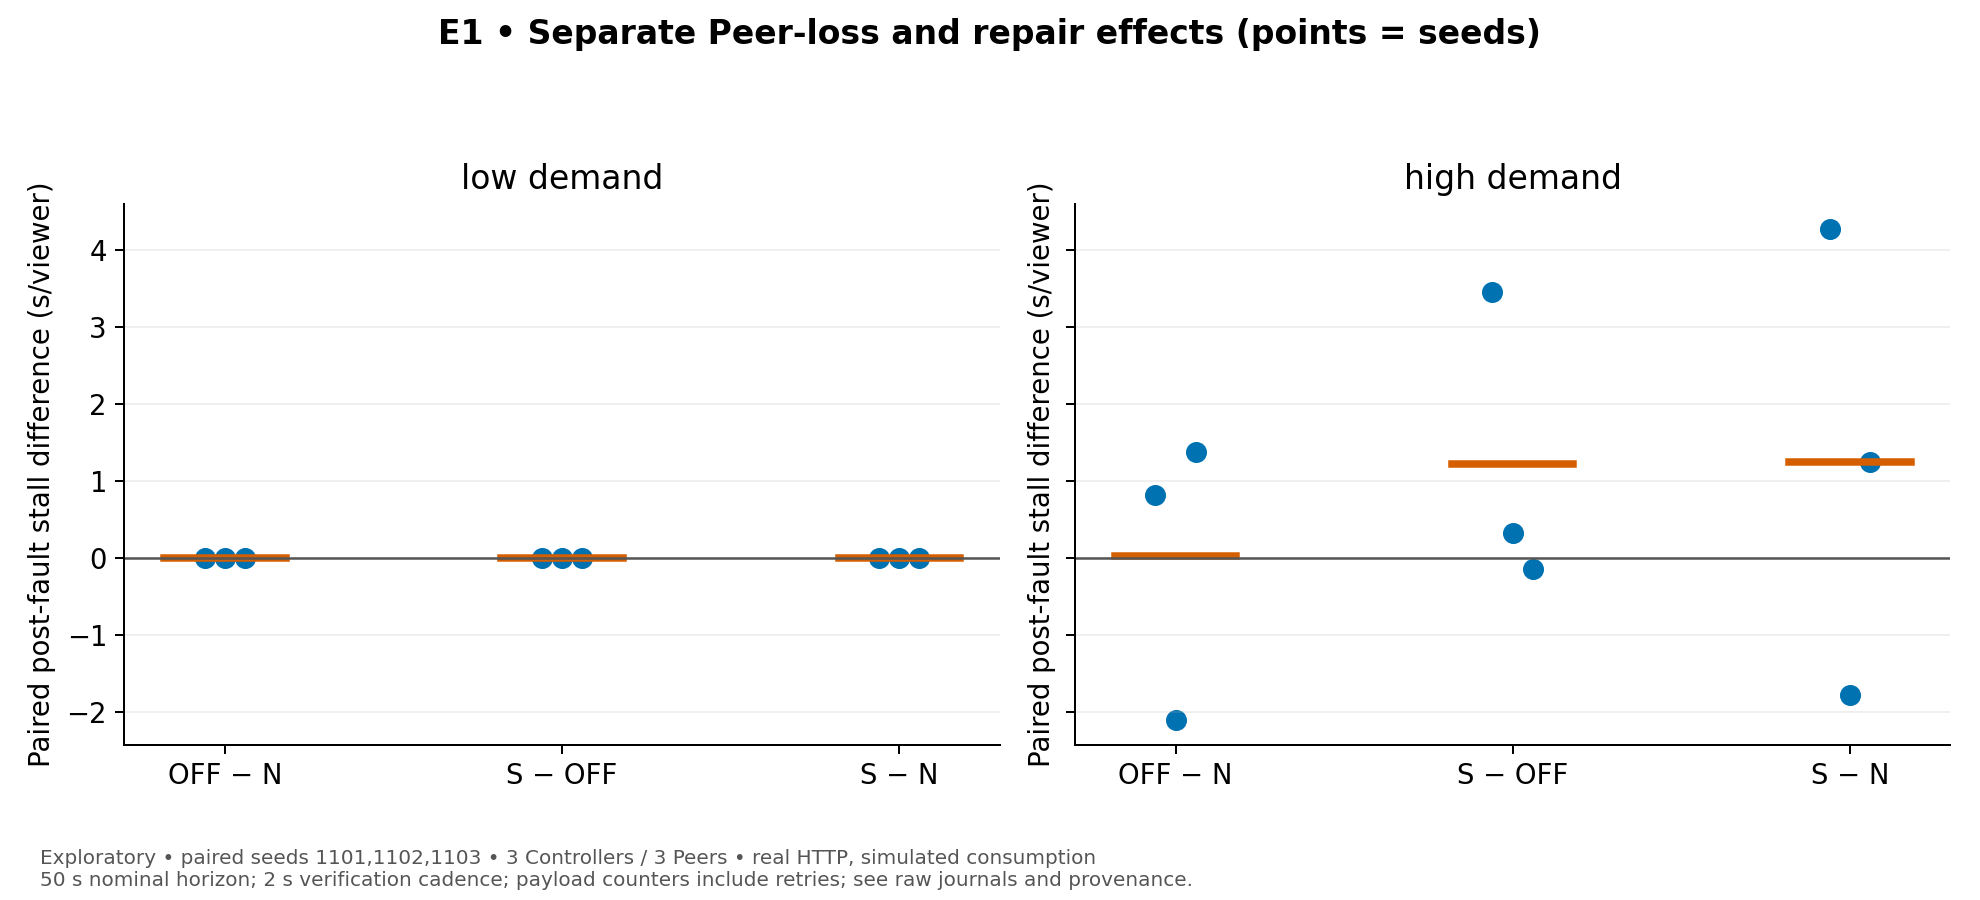
\includegraphics[width=\textwidth,height=.70\textheight,keepaspectratio]{E1-paired-effects.png}
\note{Early failed sessions can report lower observed stalls; show completion alongside this plot. Source: archived E1 paired effects.}
\end{frame}
\begin{frame}{E3: outcomes by failed source capacity}
\centering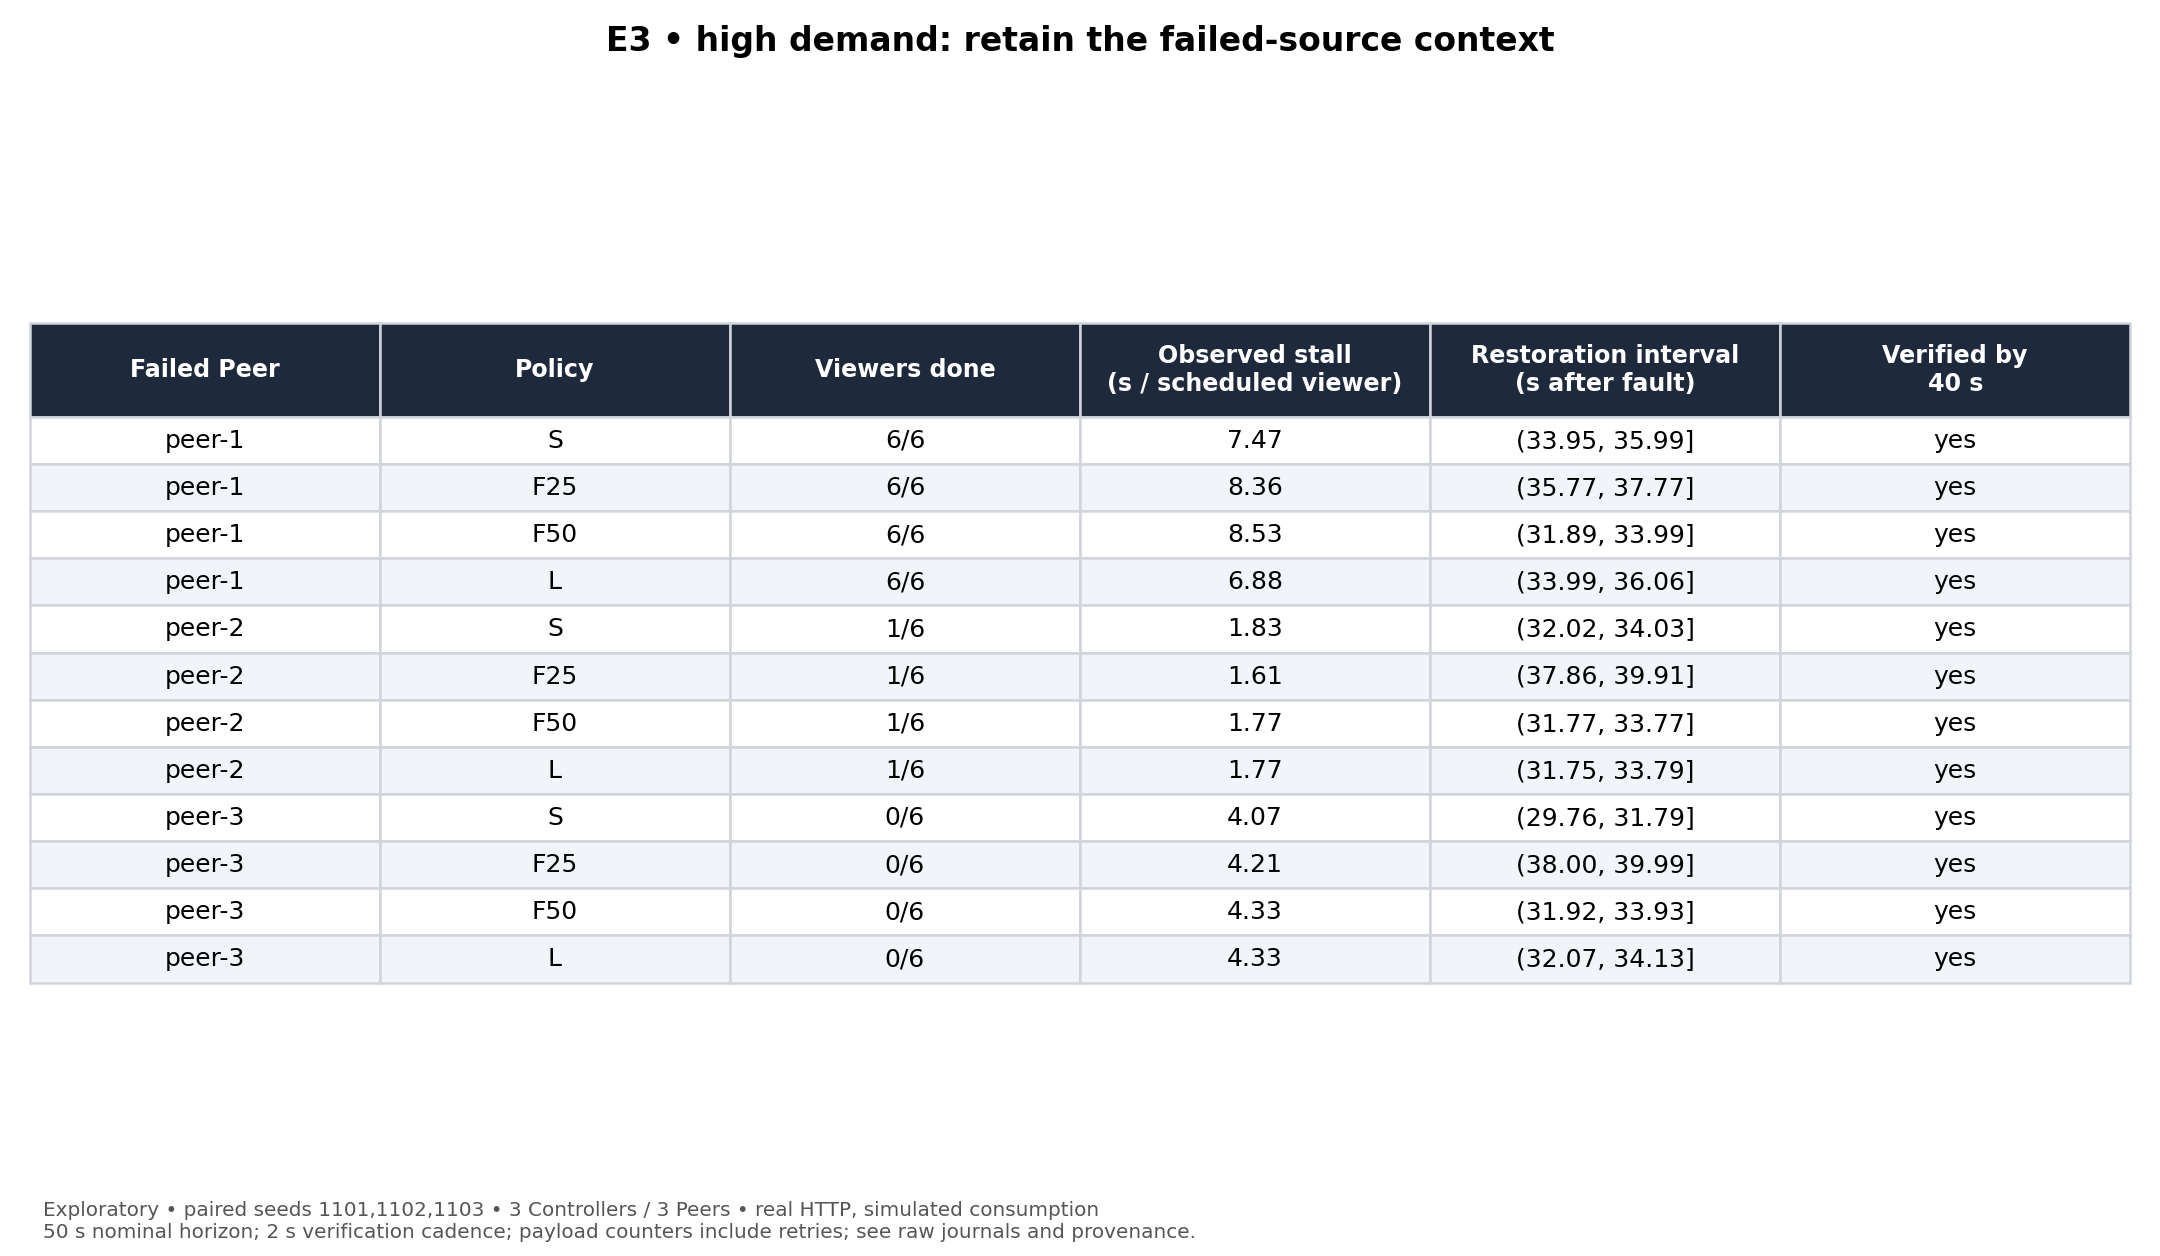
\includegraphics[width=\textwidth,height=.70\textheight,keepaspectratio]{E3-high-by-failed-peer.png}
\note{One paired context per failed capacity. These rows are not repeated capacity-stratum estimates.}
\end{frame}
\begin{frame}{L: recorded repair-budget behavior}
\centering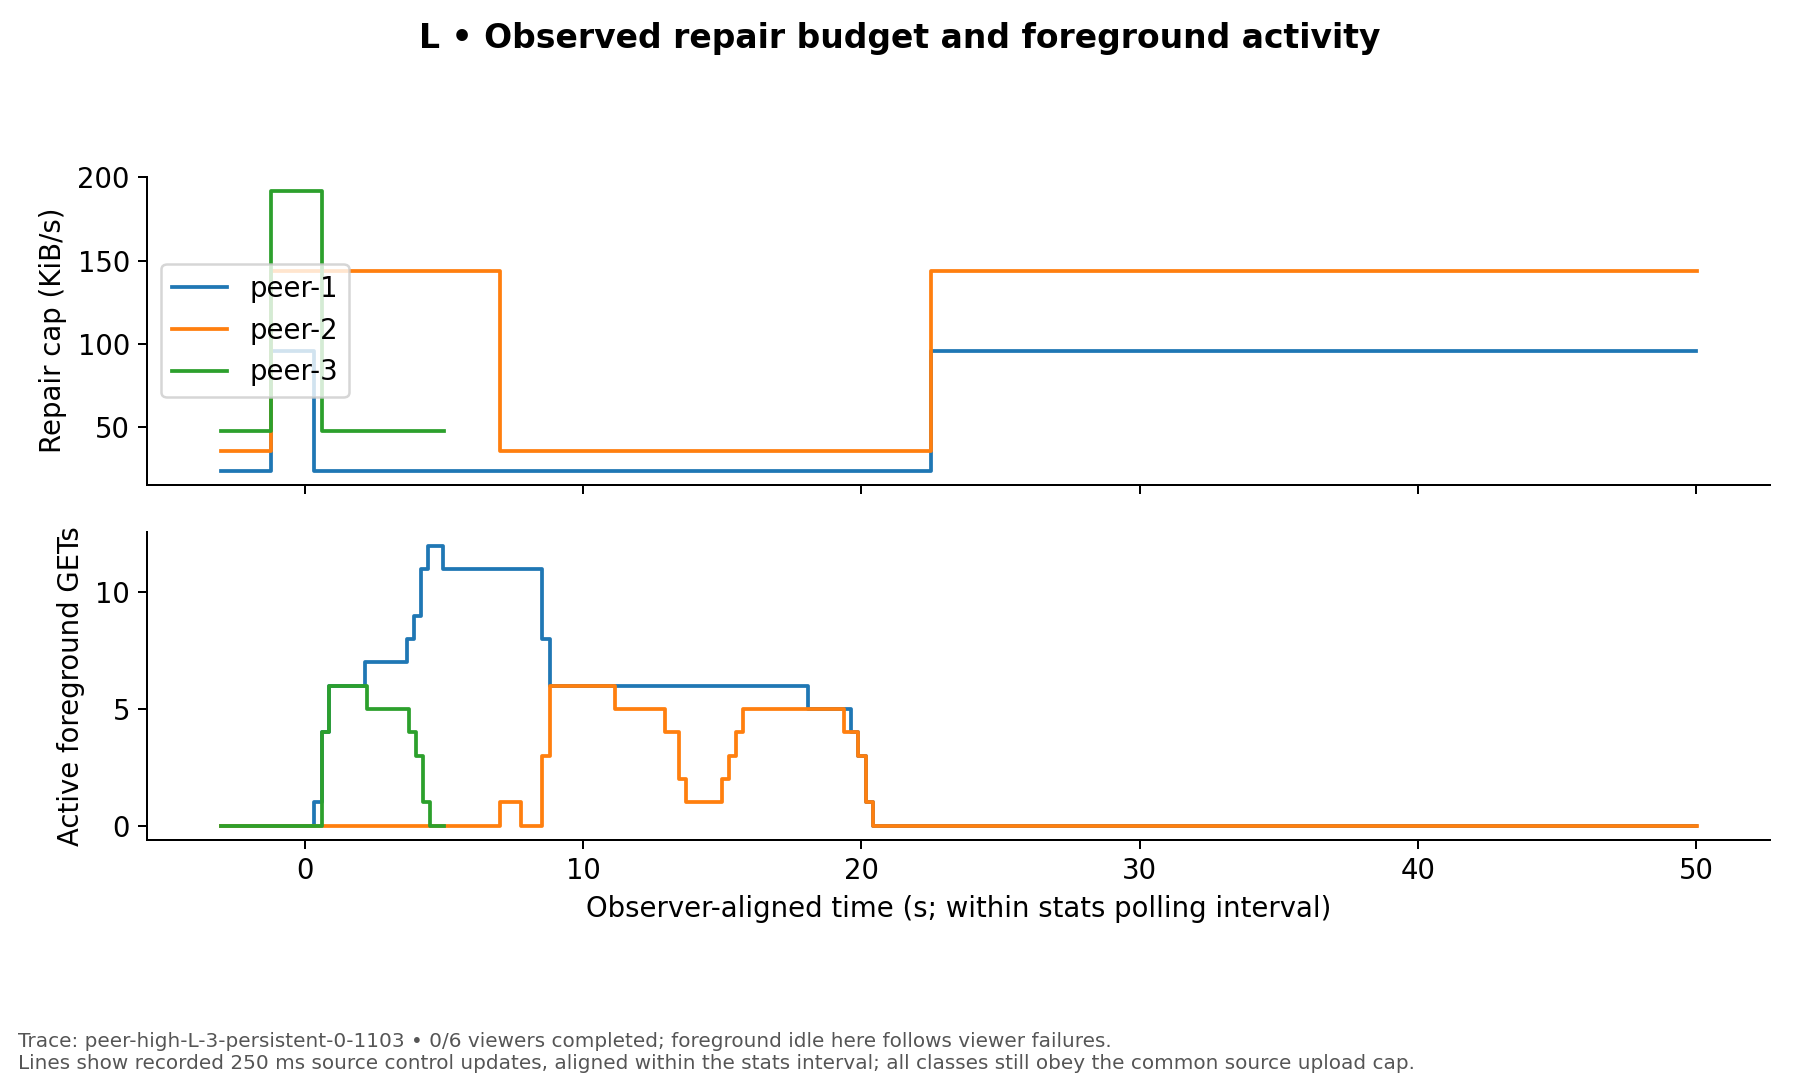
\includegraphics[width=\textwidth,height=.70\textheight,keepaspectratio]{L-budget-trace.png}
\note{This illustrated seed has 0/6 viewer completion. Idle follows failed viewers, not successful playback. The age floor did not activate during the compact performance runs.}
\end{frame}
\begin{frame}{E5: fault-relative recovery distribution}
\centering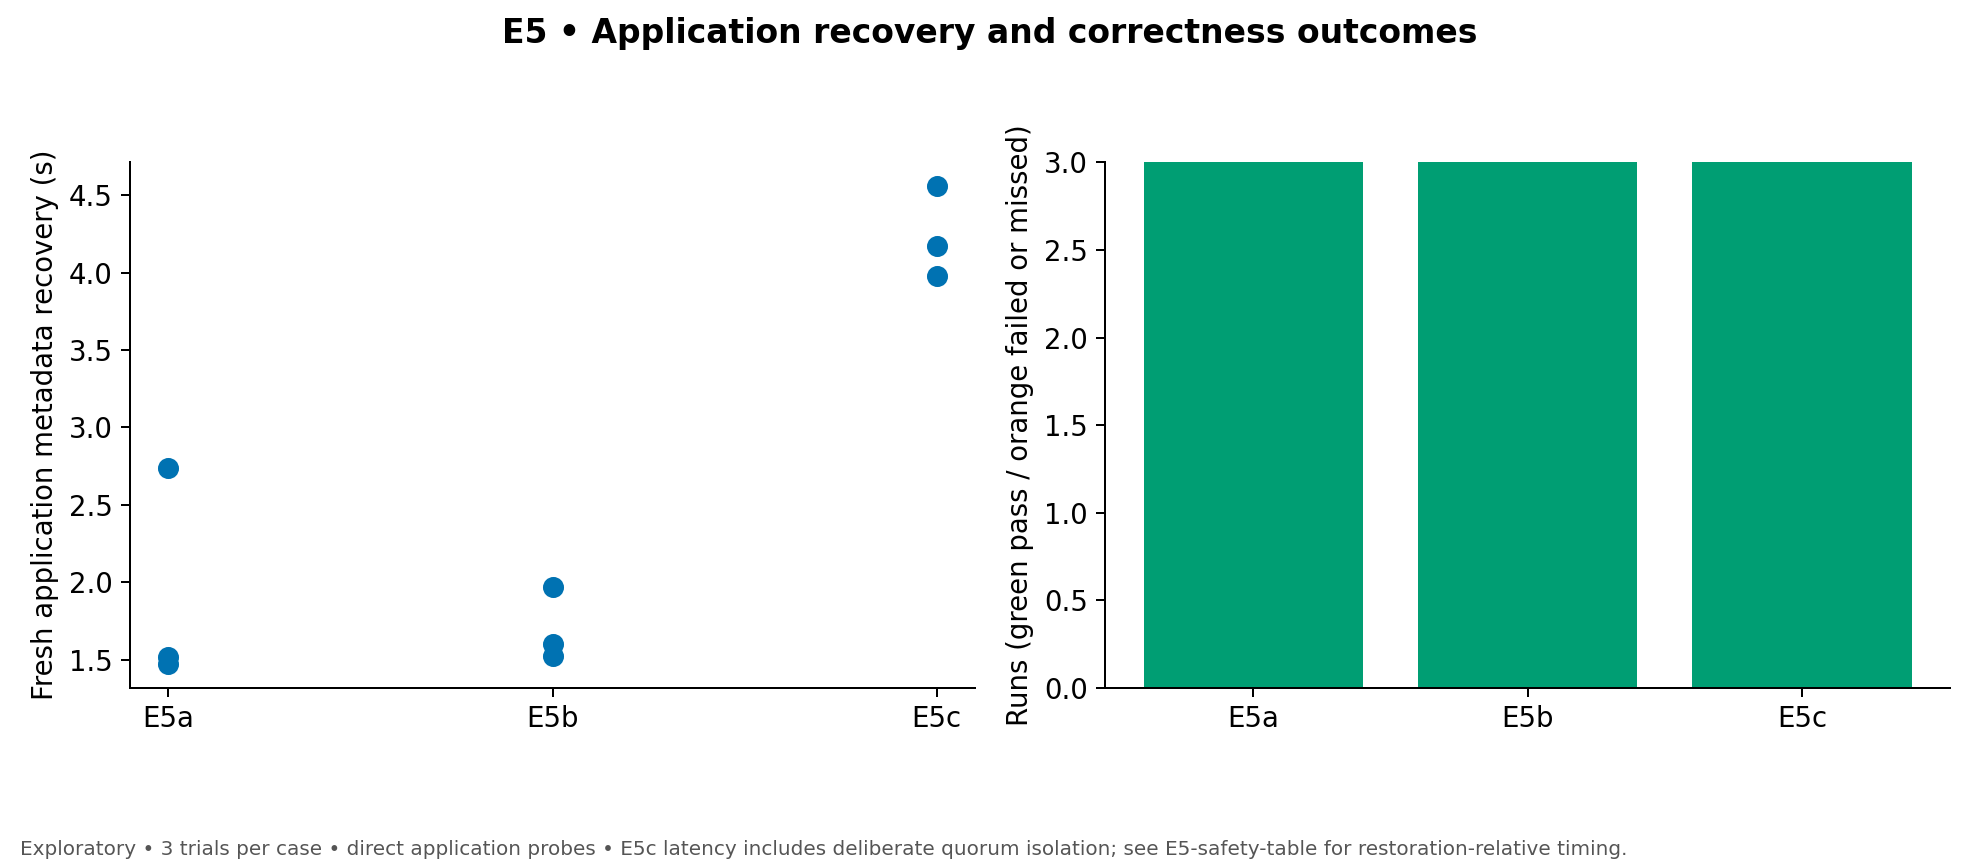
\includegraphics[width=\textwidth,height=.70\textheight,keepaspectratio]{E5-controller.png}
\note{This plot retains deliberate isolation in E5c. The main E5 table instead uses quorum-restoration-relative timing. Do not compare the two timing origins as if identical.}
\end{frame}

\end{document}
